\clearpage
\section{Thực nghiệm và đánh giá}

\subsection{Thiết lập thực nghiệm}

Nhóm đánh giá bốn thuật toán BFS, DFS, UCS và A* trên cùng
bộ 15 màn chơi được lưu dưới dạng JSON. Các thuật toán sử dụng
chung mô hình chuyển trạng thái và cùng quy tắc chi phí
$1$--$2$--$4$ đã trình bày trong phần mô hình hóa.

Repo Bloxorz AI HCMUS mô tả 12 màn. Đồ án chỉ tham khảo mã nguồn
và dữ liệu của 10 màn trong repo này, đồng thời bổ sung 5 màn mới,
tạo thành bộ 15 màn được đánh giá trong báo cáo~\cite{reference-game}.

Script \texttt{experiments/search\_experiment.py} chạy các
thuật toán, kiểm tra lời giải và xuất kết quả thành CSV cùng
các biểu đồ so sánh. Hai tệp CSV kết quả đi kèm đồ án gồm 60 dòng,
tương ứng với 15 màn chơi và 4 thuật toán.

Báo cáo sử dụng hai tệp CSV chi tiết và tổng hợp kèm theo đồ án. Dữ liệu chứa số đo của 15 màn và bốn thuật toán; không lưu cấu hình CPU, RAM, hệ điều hành, phiên bản môi trường hay số lượt đo đã sử dụng. Vì vậy, các giá trị thời gian chỉ được diễn giải trong phạm vi bộ kết quả này.

Trước khi đo, script chạy khởi động các thuật toán trên bộ test.
Script lấy trung vị thời gian theo số lượt cấu hình bằng tham số \texttt{--runs}, mặc định là 5.
Bộ nhớ được đo bằng một lượt chạy riêng để tránh ảnh hưởng
của việc theo dõi cấp phát bộ nhớ lên phép đo thời gian.

\subsection{Phân nhóm màn chơi}

Bộ test được chia thành bốn nhóm theo các loại ô xuất hiện
trong bản đồ.

\begin{table}[htbp]
\centering
\small
\caption{Phân nhóm bộ test}
\begin{tabularx}{\linewidth}{|l|p{3.6cm}|X|}
\hline
Nhóm & Màn chơi & Đặc điểm \\\hline
Cơ bản
& 1, 2, 3
& Không có fragile, công tắc hoặc cầu. \\\hline
Fragile
& 14, 15
& Có fragile, không có công tắc hoặc cầu. \\\hline
Switch
& 4, 5, 6, 7, 10
& Có công tắc hoặc cầu, không có fragile. \\\hline
Kết hợp
& 8, 9, 11, 12, 13
& Có cả fragile và công tắc hoặc cầu. \\\hline
\end{tabularx}
\end{table}

Các màn 6, 9 và 10 có cơ chế split trong bộ mã nguồn được
đối chiếu. Phân nhóm dựa trên loại ô có trong bản đồ,
không có nghĩa mỗi lời giải bắt buộc sử dụng tất cả các ô
đặc biệt đó.

Độ khó tìm kiếm không được xác định chỉ bằng số thứ tự màn
hoặc số hành động của lời giải. Cấu trúc bản đồ, số nhánh,
trạng thái cầu và vị trí hai cube khi tách đều ảnh hưởng
đến số trạng thái cần khảo sát.

\subsection{Chỉ số đánh giá và phương pháp đo}

\begin{enumerate}

\item \textbf{Thời gian tìm kiếm (ms):}
được đo bằng \texttt{perf\_counter} và lấy trung vị của các lượt chạy theo cấu hình script. Các lượt đo thời gian không bật
\texttt{tracemalloc}. Thời gian bao gồm thao tác bên trong
solver, kể cả dựng lại đường đi và tính chi phí lời giải,
nhưng không gồm tải JSON hoặc vẽ biểu đồ.

\item \textbf{Bộ nhớ đỉnh (KiB):}
được đo bằng \texttt{tracemalloc} trong một lượt chạy riêng.
Đây là bộ nhớ Python được theo dõi, không phải tổng RAM
của tiến trình, toàn bộ máy hoặc bộ nhớ GPU.
Script chuyển giá trị MiB của profiler sang KiB bằng cách
nhân với $1024$.

\item \textbf{Số nút mở rộng (Expanded nodes):}
là số mục trạng thái hợp lệ được lấy ra khỏi frontier
để xử lý. Theo quy ước cài đặt, số đếm bao gồm nút đích.
Các mục heap cũ không còn tương ứng với chi phí tốt nhất
được bỏ qua.

\item \textbf{Độ dài lời giải (Length):}
là số hành động trong đường đi, bao gồm hành động đổi cube
đang điều khiển khi khối tách.

\item \textbf{Tổng chi phí lời giải (Cost):}
là tổng chi phí $1$--$2$--$4$ của các hành động trên
đường đi tìm được.

\end{enumerate}

Số successor được sinh ra, ký hiệu Generated, cũng được lưu
trong CSV để hỗ trợ kiểm tra. Chỉ số này được tăng trước khi
lọc trạng thái lặp nên không phải số trạng thái phân biệt.

Thời gian trong bảng Results của game được đo khi bật theo dõi
bộ nhớ, nên có thể khác thời gian trong CSV. Báo cáo sử dụng
nhất quán số liệu từ script thực nghiệm. Các giá trị được
trình bày theo độ làm tròn của CSV, không hàm ý phép đo có
độ chính xác thống kê tương ứng.

\subsection{Kiểm tra tính hợp lệ của lời giải}

Script chạy lại từng lời giải từ trạng thái đầu bằng
\texttt{apply\_move}. Một lời giải hợp lệ phải không chứa
hành động bị từ chối và kết thúc tại trạng thái thỏa
điều kiện thắng.

Chi phí được cộng lại dọc đường đi và đối chiếu với
\texttt{solution\_cost} mà solver trả về. Kết quả cho thấy
cả 60 dòng đều có \texttt{success=True},
\texttt{valid=True} và \texttt{cost\_valid=True}.
Giá trị Cost bằng Checked cost trong tất cả trường hợp.

Đối chiếu giữa các thuật toán trên cùng màn cho thấy:

\[
C_{\mathrm{UCS}}=C_{\mathrm{A*}},
\]

\[
C_{\mathrm{UCS}}\le C_{\mathrm{BFS}},
\qquad
C_{\mathrm{UCS}}\le C_{\mathrm{DFS}},
\]

\[
L_{\mathrm{BFS}}\le L_{\mathrm{UCS}},
\qquad
L_{\mathrm{BFS}}\le L_{\mathrm{A*}},
\qquad
L_{\mathrm{BFS}}\le L_{\mathrm{DFS}}.
\]

Các quan hệ trên đều thỏa trên bộ 15 màn. Kết quả phù hợp với
mục tiêu tối ưu của từng thuật toán. Tuy nhiên, kiểm tra replay
sử dụng cùng mô hình chuyển trạng thái với solver nên chưa
thay thế việc kiểm thử độc lập các luật game, đặc biệt là
các trường hợp biên của split.

\subsection{Kết quả trên từng màn chơi}

\begin{table}[htbp]
\centering
\small
\caption{Độ dài lời giải theo từng màn, đơn vị hành động}
\begin{tabular}{|r|r|r|r|r|}
\hline
Màn & BFS & DFS & UCS & A* \\\hline
1  & 8   & 28   & 9   & 9   \\\hline
2  & 19  & 32   & 19  & 19  \\\hline
3  & 35  & 51   & 35  & 35  \\\hline
4  & 32  & 110  & 32  & 32  \\\hline
5  & 44  & 69   & 44  & 44  \\\hline
6  & 11  & 149  & 11  & 11  \\\hline
7  & 22  & 66   & 22  & 22  \\\hline
8  & 30  & 35   & 30  & 30  \\\hline
9  & 45  & 305  & 45  & 45  \\\hline
10 & 58  & 1276 & 58  & 58  \\\hline
11 & 94  & 94   & 94  & 94  \\\hline
12 & 110 & 110  & 110 & 110 \\\hline
13 & 126 & 126  & 126 & 126 \\\hline
14 & 39  & 39   & 39  & 39  \\\hline
15 & 32  & 70   & 32  & 32  \\\hline
\end{tabular}
\end{table}

\begin{table}[htbp]
\centering
\small
\caption{Tổng chi phí lời giải theo từng màn}
\begin{tabular}{|r|r|r|r|r|}
\hline
Màn & BFS & DFS & UCS & A* \\\hline
1  & 12  & 44   & 11  & 11  \\\hline
2  & 33  & 52   & 33  & 33  \\\hline
3  & 57  & 85   & 57  & 57  \\\hline
4  & 52  & 186  & 52  & 52  \\\hline
5  & 76  & 119  & 76  & 76  \\\hline
6  & 17  & 175  & 17  & 17  \\\hline
7  & 38  & 110  & 38  & 38  \\\hline
8  & 80  & 89   & 80  & 80  \\\hline
9  & 81  & 393  & 81  & 81  \\\hline
10 & 74  & 1320 & 74  & 74  \\\hline
11 & 192 & 192  & 192 & 192 \\\hline
12 & 222 & 222  & 222 & 222 \\\hline
13 & 258 & 258  & 258 & 258 \\\hline
14 & 122 & 122  & 122 & 122 \\\hline
15 & 62  & 128  & 62  & 62  \\\hline
\end{tabular}
\end{table}

\clearpage

\begin{table}[htbp]
\centering
\small
\caption{Số nút mở rộng theo từng màn}
\begin{tabular}{|r|r|r|r|r|}
\hline
Màn & BFS & DFS & UCS & A* \\\hline
1  & 81    & 36   & 68    & 32    \\\hline
2  & 98    & 100  & 98    & 89    \\\hline
3  & 107   & 78   & 110   & 107   \\\hline
4  & 384   & 179  & 380   & 376   \\\hline
5  & 177   & 153  & 178   & 177   \\\hline
6  & 824   & 161  & 1494  & 1494  \\\hline
7  & 283   & 87   & 286   & 254   \\\hline
8  & 123   & 101  & 112   & 99    \\\hline
9  & 1578  & 2936 & 1675  & 1675  \\\hline
10 & 10671 & 1602 & 12722 & 12722 \\\hline
11 & 101   & 95   & 101   & 101   \\\hline
12 & 129   & 125  & 129   & 129   \\\hline
13 & 225   & 127  & 224   & 217   \\\hline
14 & 55    & 77   & 55    & 55    \\\hline
15 & 244   & 179  & 242   & 238   \\\hline
\end{tabular}
\end{table}

\begin{table}[htbp]
\centering
\small
\caption{Trung vị thời gian tìm kiếm theo từng màn, đơn vị ms}
\begin{tabular}{|r|r|r|r|r|}
\hline
Màn & BFS & DFS & UCS & A* \\\hline
1  & 2.502   & 1.197   & 2.546   & 1.332   \\\hline
2  & 2.934   & 3.524   & 3.456   & 3.370   \\\hline
3  & 3.142   & 2.337   & 3.657   & 3.853   \\\hline
4  & 11.360  & 5.428   & 13.186  & 13.654  \\\hline
5  & 4.961   & 4.549   & 6.995   & 7.778   \\\hline
6  & 31.979  & 6.270   & 68.878  & 67.145  \\\hline
7  & 9.292   & 3.008   & 10.854  & 11.145  \\\hline
8  & 3.557   & 2.941   & 3.699   & 3.509   \\\hline
9  & 56.011  & 109.279 & 70.527  & 81.483  \\\hline
10 & 389.705 & 59.801  & 527.138 & 553.506 \\\hline
11 & 2.745   & 2.671   & 2.982   & 3.263   \\\hline
12 & 3.429   & 3.380   & 3.914   & 4.159   \\\hline
13 & 5.969   & 3.399   & 6.615   & 6.973   \\\hline
14 & 1.530   & 2.126   & 1.718   & 1.897   \\\hline
15 & 8.379   & 5.962   & 9.025   & 9.576   \\\hline
\end{tabular}
\end{table}

\clearpage

\begin{table}[htbp]
\centering
\small
\caption{Bộ nhớ Python đỉnh theo từng màn, đơn vị KiB}
\begin{tabular}{|r|r|r|r|r|}
\hline
Màn & BFS & DFS & UCS & A* \\\hline
1  & 34.457   & 18.012   & 23.441   & 16.402   \\\hline
2  & 37.738   & 39.137   & 33.223   & 31.426   \\\hline
3  & 38.324   & 32.762   & 34.332   & 34.098   \\\hline
4  & 132.371  & 64.988   & 114.270  & 114.461  \\\hline
5  & 57.309   & 55.648   & 56.871   & 56.637   \\\hline
6  & 275.738  & 128.367  & 565.348  & 565.316  \\\hline
7  & 81.652   & 42.434   & 82.465   & 74.664   \\\hline
8  & 41.691   & 37.660   & 35.387   & 32.160   \\\hline
9  & 612.105  & 1314.402 & 601.070  & 601.086  \\\hline
10 & 5246.133 & 1260.461 & 5779.180 & 5754.320 \\\hline
11 & 36.035   & 34.246   & 31.551   & 31.512   \\\hline
12 & 41.465   & 39.910   & 36.824   & 36.785   \\\hline
13 & 65.973   & 40.902   & 64.957   & 63.293   \\\hline
14 & 18.520   & 29.582   & 18.012   & 17.973   \\\hline
15 & 72.277   & 66.285   & 72.012   & 71.859   \\\hline
\end{tabular}
\end{table}

\begin{table}[htbp]
\centering
\small
\caption{Kết quả trung bình trên toàn bộ 15 màn}
\begin{tabular}{|l|r|r|r|r|r|}
\hline
Thuật toán & Length & Cost & Expanded & Time (ms) & Memory (KiB) \\\hline
BFS & 47.000  & 91.733  & 1005.333 & 35.833 & 452.786 \\\hline
DFS & 170.667 & 233.000 & 402.400  & 14.392 & 213.653 \\\hline
UCS & 47.067  & 91.667  & 1191.600 & 49.013 & 503.263 \\\hline
A*  & 47.067  & 91.667  & 1184.333 & 51.509 & 500.133 \\\hline
\end{tabular}
\end{table}

Các số trung bình trong bảng được lấy trên toàn bộ 15 màn.
Đối với thời gian, đây là trung bình cộng của các thời gian
trung vị theo từng màn, không phải trung vị chung của mọi
lượt chạy.

\clearpage
\subsection{Biểu đồ so sánh}

Các biểu đồ sử dụng thang log để thể hiện các giá trị có
độ lớn chênh lệch. Trên thang log, khoảng cách giữa các
giá trị phản ánh tỷ lệ, không phải chênh lệch tuyệt đối.

\begin{figure}[H]\centering
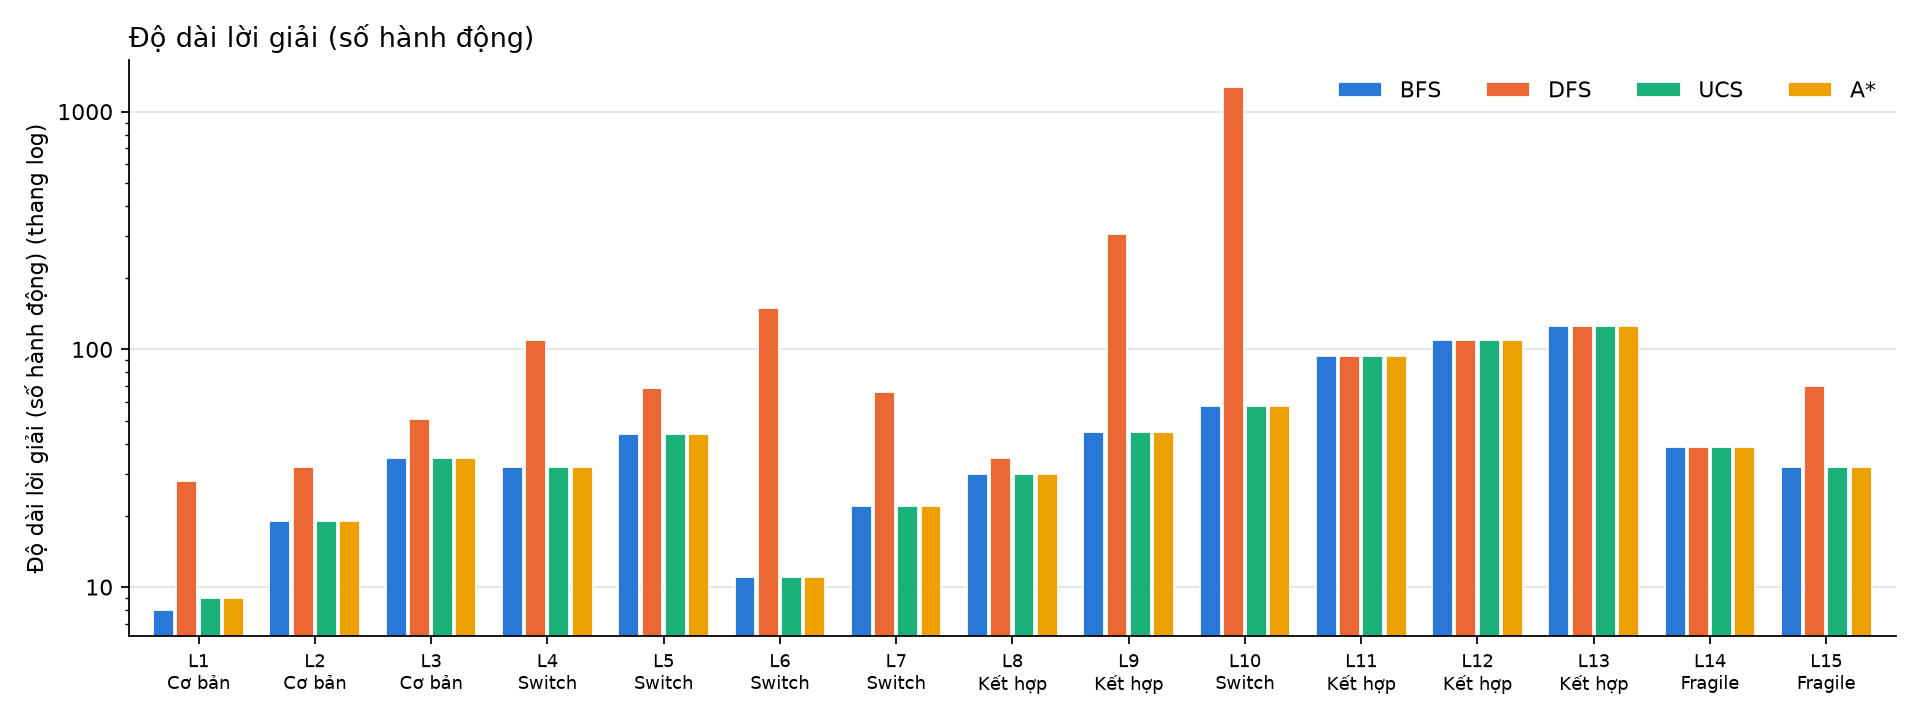
\includegraphics[width=1.0\linewidth]{figures/length.png}
\caption{So sánh độ dài lời giải trên 15 màn.}\end{figure}
\begin{figure}[H]\centering
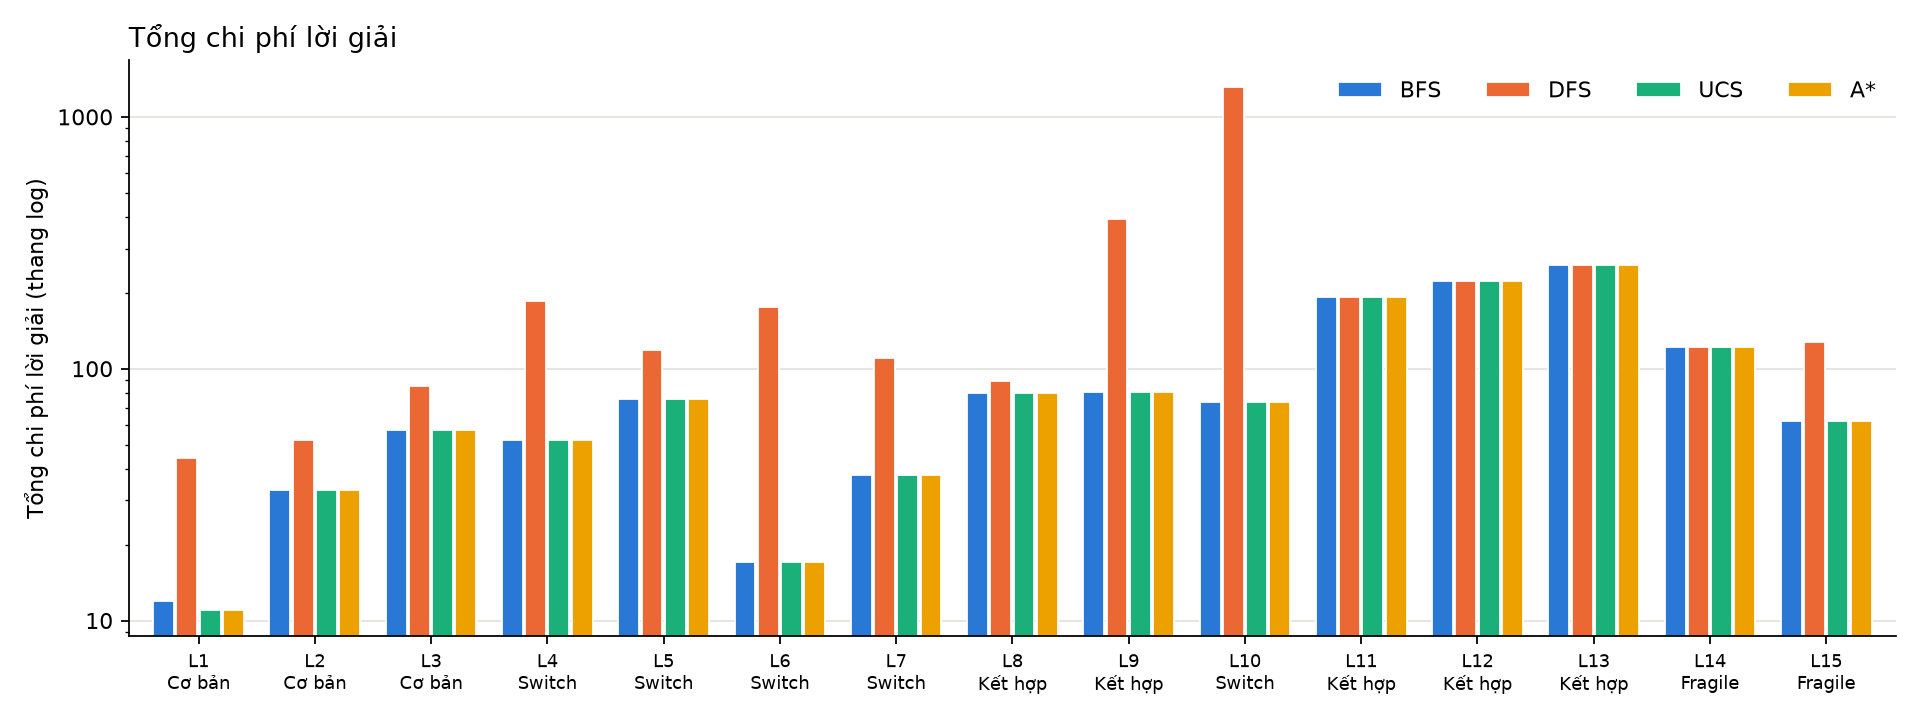
\includegraphics[width=1.0\linewidth]{figures/cost.png}
\caption{So sánh tổng chi phí lời giải theo quy tắc $1$--$2$--$4$.}\end{figure}
\clearpage
\begin{figure}[H]\centering
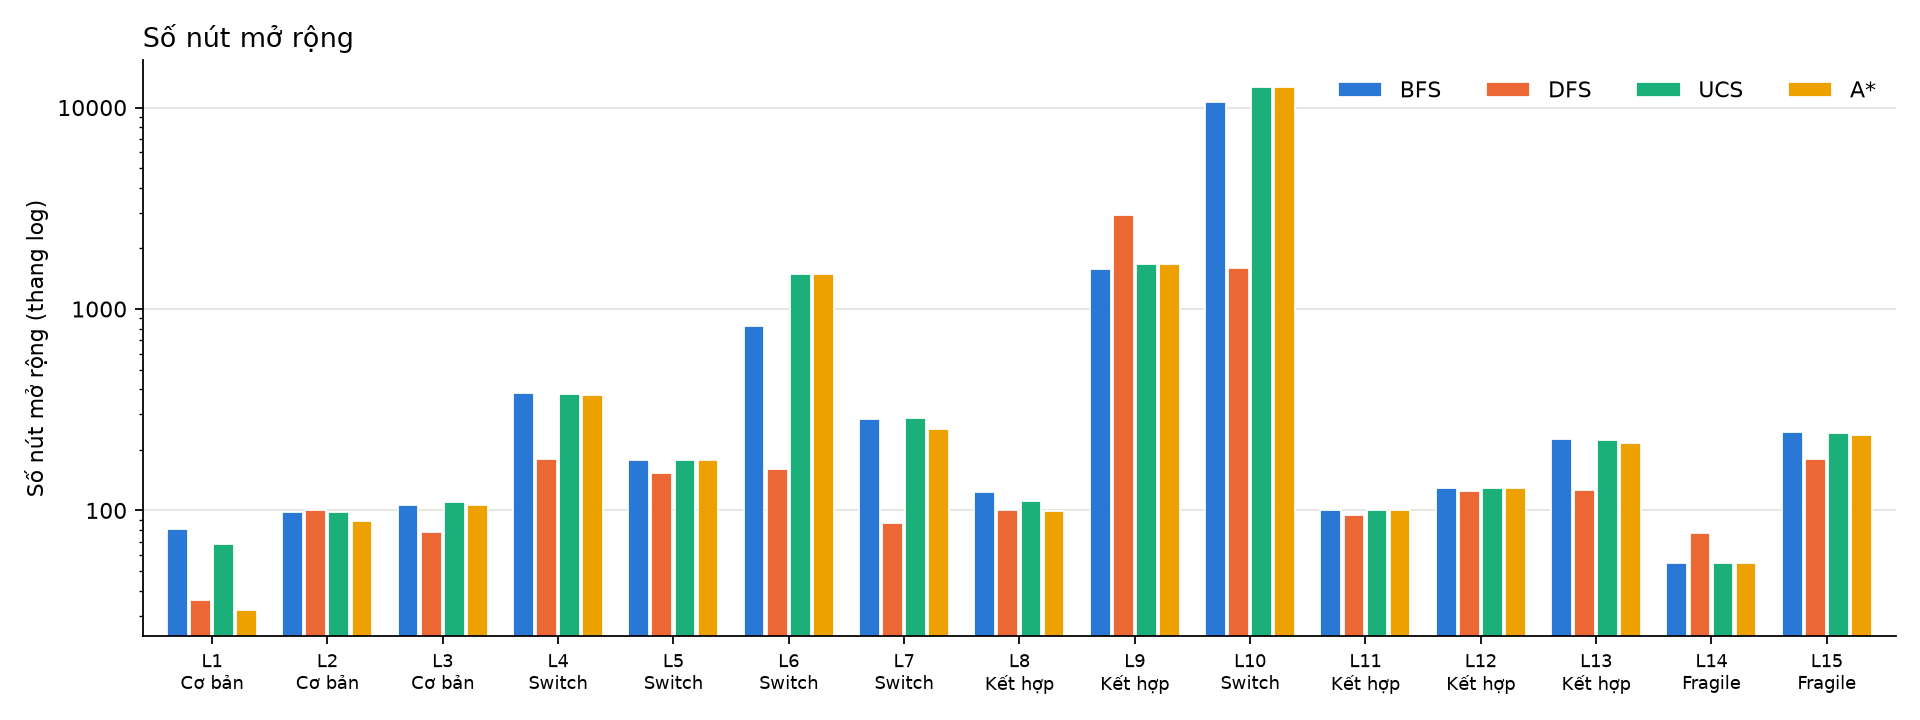
\includegraphics[width=1.0\linewidth]{figures/expanded.png}
\caption{So sánh số nút mở rộng trên từng màn.}\end{figure}
\begin{figure}[H]\centering
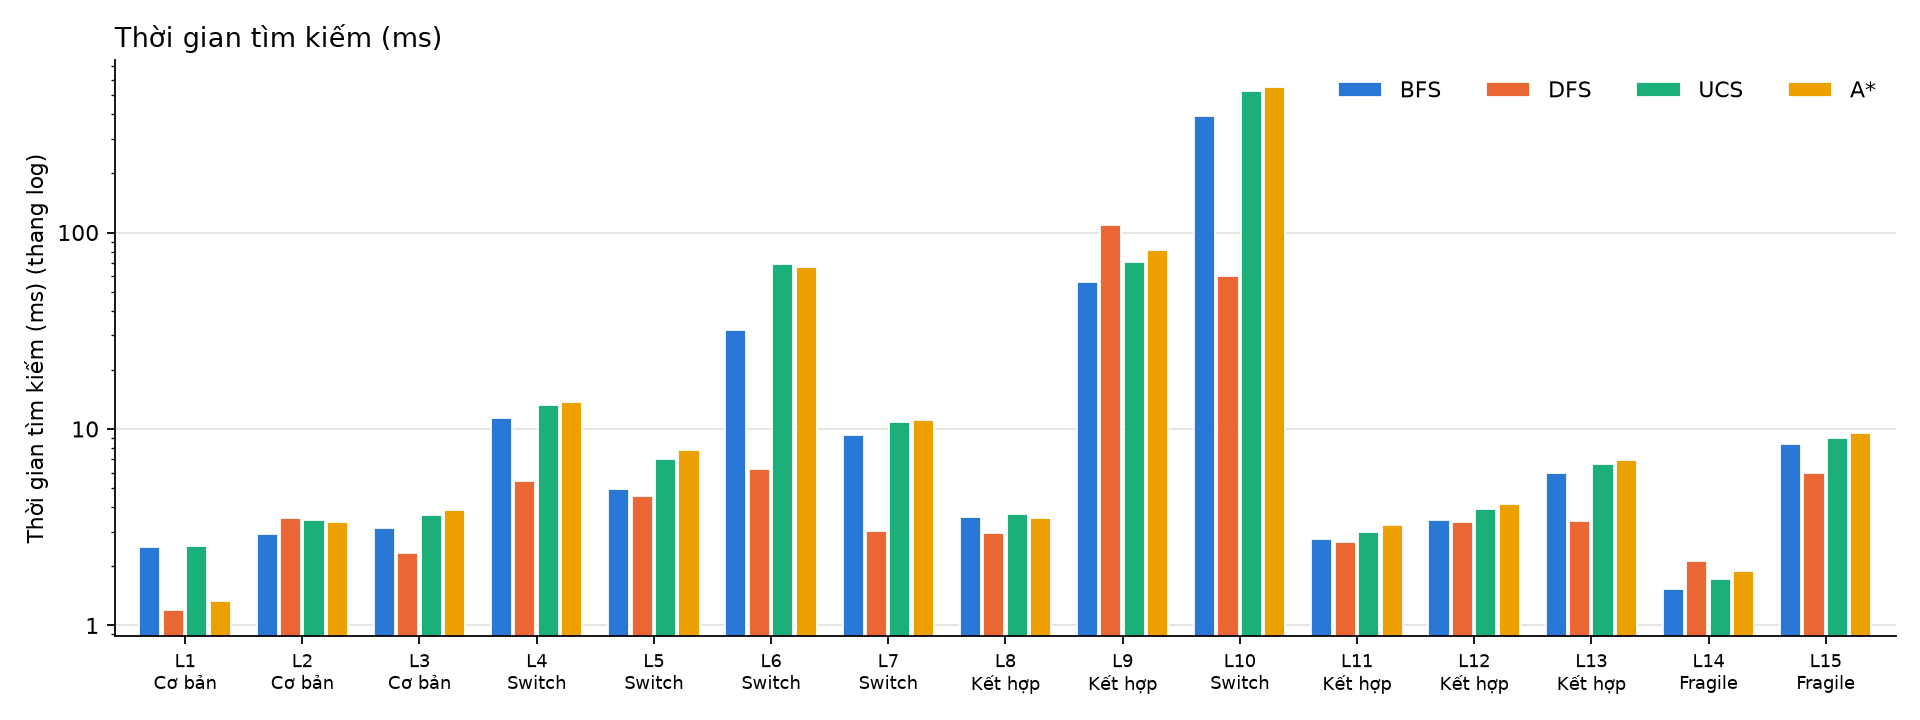
\includegraphics[width=1.0\linewidth]{figures/time.png}
\caption{Trung vị thời gian tìm kiếm theo từng màn, đơn vị ms.}
\caption*{Lưu ý: Trung vị thời gian có thể khác nhau giữa các lần đo tùy theo tình trạng hoạt động của máy.}\end{figure}
\clearpage
\begin{figure}[H]\centering
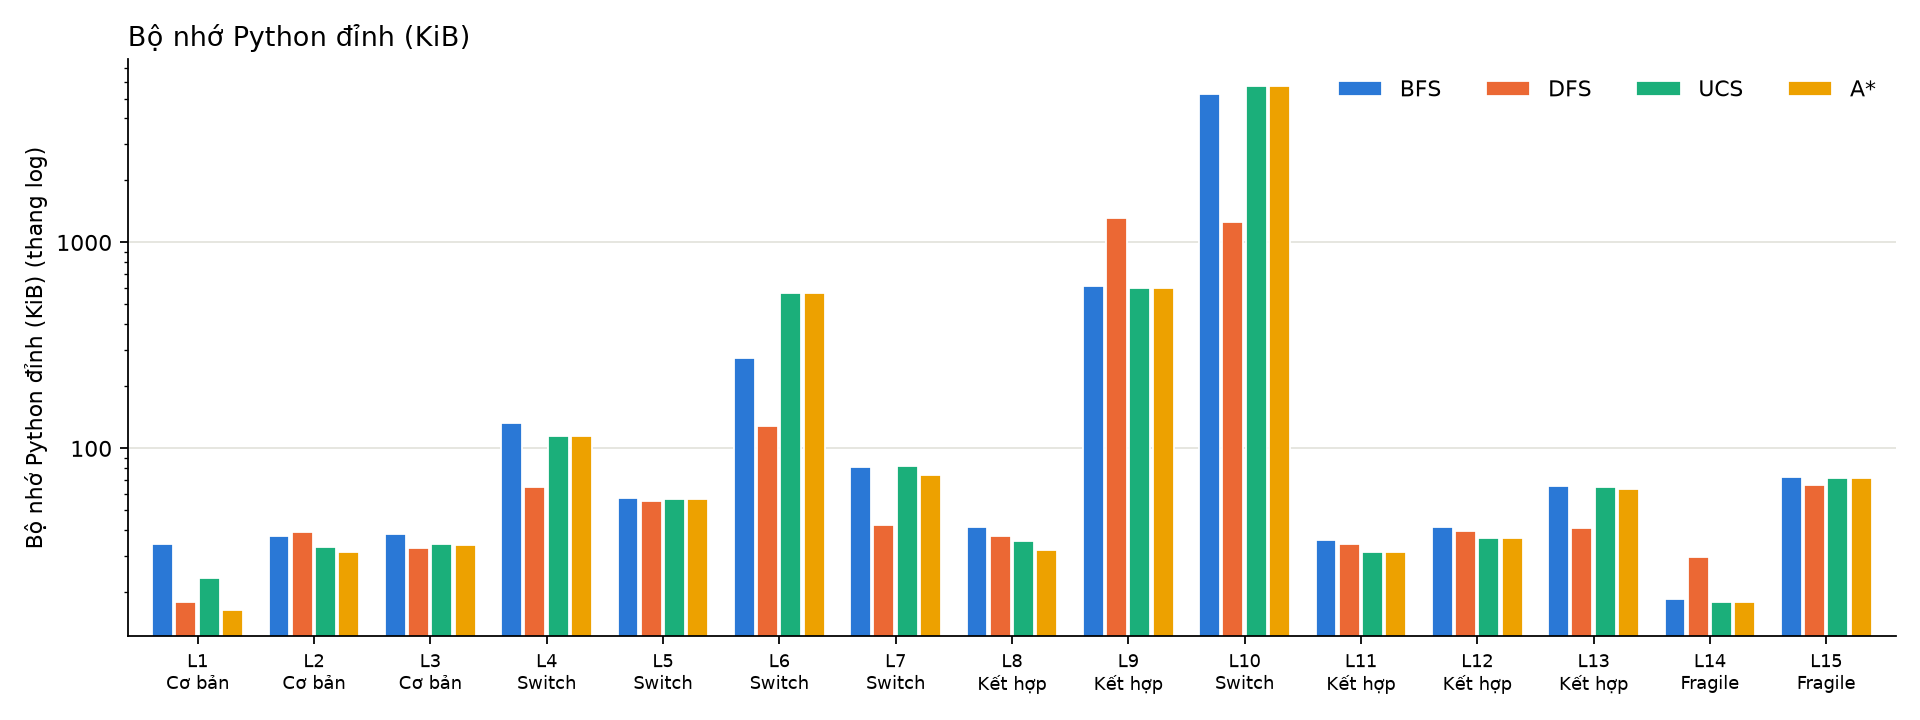
\includegraphics[width=1.0\linewidth]{figures/memory.png}
\caption{Bộ nhớ Python đỉnh theo từng màn, đơn vị KiB.}\end{figure}
\begin{figure}[H]\centering
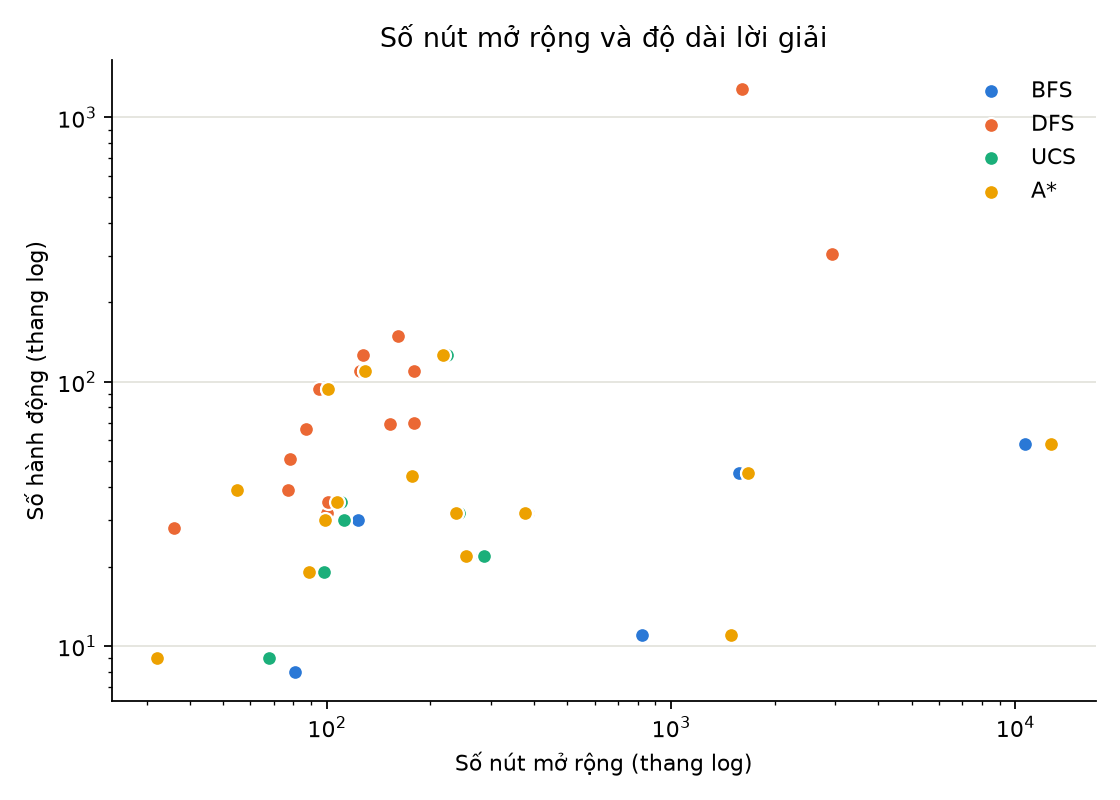
\includegraphics[width=0.80\linewidth]{figures/tradeoff.png}
\caption{Quan hệ giữa số nút mở rộng và số hành động của lời giải.}\end{figure}
\clearpage
\subsection{Phân tích kết quả}

\subsubsection{Độ dài và tổng chi phí lời giải}

Màn 1 minh họa rõ sự khác nhau giữa tối ưu số hành động và
tối ưu chi phí. BFS tìm lời giải gồm 8 hành động với Cost 12.
Trong khi đó, UCS và A* tìm lời giải gồm 9 hành động nhưng
Cost chỉ bằng 11. Như vậy, thêm một hành động giúp giảm
một đơn vị chi phí, tương đương khoảng $8.33\%$ so với
chi phí của đường BFS.

Kết quả này phù hợp với mục tiêu của các thuật toán:
BFS tối thiểu hóa số hành động, còn UCS và A* tối thiểu hóa
tổng trọng số. Vì vậy không thể kết luận UCS hoặc A* kém hơn
BFS chỉ vì đường đi có nhiều hành động hơn.

Ở 14 màn còn lại, BFS, UCS và A* có cùng Length và Cost.
Sự trùng số đo không chứng minh chuỗi hành động giống nhau
vì CSV không lưu đường đi cụ thể. Chi phí trung bình của BFS
là $91.733$, còn UCS và A* là $91.667$. Chênh lệch nhỏ do
bộ test hiện chỉ có màn 1 thể hiện khác biệt về chi phí
giữa các lời giải được trả về.

DFS có Length trung bình $170.667$ và Cost trung bình
$233.000$, cao hơn ba thuật toán còn lại. Trường hợp rõ nhất
là màn 10: DFS cần 1276 hành động với Cost 1320, trong khi
BFS, UCS và A* chỉ cần 58 hành động với Cost 74.
Đường đi DFS dài gấp $22$ lần và đắt khoảng $17.84$ lần.

Ở các màn 11, 12, 13 và 14, cả bốn thuật toán có cùng Length
và Cost. Tuy nhiên, chỉ từ kết quả này chưa thể khẳng định
mỗi màn chỉ có một đường tới đích.

\subsubsection{Hiệu quả của heuristic A*}

Ở màn 1 không có split, A* mở rộng 32 nút so với 68 nút
của UCS, giảm khoảng $52.94\%$. Thời gian tìm kiếm giảm từ
$2.546$ ms xuống $1.332$ ms, tương ứng khoảng $47.68\%$
trong lần đo này. Bộ nhớ cũng giảm từ $23.441$ KiB xuống
$16.402$ KiB.

Tuy nhiên, giảm số nút không luôn làm thời gian giảm.
Ở màn 7, A* mở 254 nút so với 286 nút của UCS, nhưng
thời gian là $11.145$ ms so với $10.854$ ms.
Ở màn 13, số nút giảm từ 224 xuống 217 nhưng thời gian
tăng từ $6.615$ ms lên $6.973$ ms.
Chi phí tính heuristic và biến động môi trường thực thi
là các khả năng giải thích; dữ liệu hiện tại chưa tách
riêng được ảnh hưởng của từng nguyên nhân.

Trên các màn split 6, 9 và 10, A* sử dụng $h=0$ nên có
chiến lược tương đương UCS. Expanded, Generated, Length
và Cost của hai thuật toán trùng nhau trên cả ba màn.
Chẳng hạn ở màn 10, cả UCS và A* đều mở rộng 12722 nút
và sinh 45981 successor.

Thời gian vẫn có thể khác dù thứ tự tìm kiếm tương đương.
Ở màn 10, UCS mất $527.138$ ms, còn A* mất $553.506$ ms.
Không xem đây là bằng chứng về hiệu quả định hướng
của heuristic vì heuristic trên màn này bằng không.

Trên toàn bộ bộ test, số nút trung bình của A* là
$1184.333$, so với $1191.600$ của UCS, chỉ giảm khoảng
$0.61\%$. Thời gian trung bình của A* là $51.509$ ms,
cao hơn UCS với $49.013$ ms. Vì vậy bộ số liệu này
không hỗ trợ kết luận A* luôn nhanh hơn UCS.

\subsubsection{BFS và UCS khi chi phí không đồng nhất}

Với trọng số $1$--$2$--$4$, thứ tự mở rộng của UCS không còn
nhất thiết giống BFS. BFS ưu tiên ít hành động từ điểm đầu,
còn UCS ưu tiên tổng chi phí đã đi nhỏ nhất.

Ở màn 6, BFS mở rộng 824 nút trong khi UCS mở rộng 1494 nút.
Ở màn 10, các giá trị tương ứng là 10671 và 12722.
UCS có thể phải khảo sát nhiều trạng thái đạt được bằng
các hành động rẻ trước khi lấy đích ra khỏi hàng đợi.
Vì vậy việc UCS mở nhiều nút hơn BFS không tự động cho thấy
thuật toán sai.

Trên toàn bộ bộ test, BFS có thời gian trung bình
$35.833$ ms và bộ nhớ trung bình $452.786$ KiB.
Hai giá trị này thấp hơn UCS, lần lượt là $49.013$ ms và
$503.263$ KiB. Đổi lại, UCS bảo đảm tối ưu tổng chi phí,
trong khi BFS bảo đảm tối ưu số hành động.
So sánh tài nguyên cần đi kèm mục tiêu tối ưu tương ứng.

\subsubsection{Đặc điểm của DFS}

DFS có thời gian trung bình thấp nhất trong lần thực nghiệm
này, bằng $14.392$ ms. Số nút và bộ nhớ trung bình cũng thấp
nhất, lần lượt là $402.400$ nút và $213.653$ KiB.
Tuy nhiên, kết quả đó đi kèm lời giải có thể dài và đắt hơn
đáng kể, như trường hợp màn 10.

Màn 9 thể hiện hiệu quả không ổn định của DFS.
DFS mở 2936 nút, dùng $1314.402$ KiB và mất $109.279$ ms;
BFS tương ứng chỉ mở 1578 nút, dùng $612.105$ KiB và mất
$56.011$ ms. DFS cũng mở nhiều nút hơn BFS ở màn 2 và 14.

Các kết quả này phù hợp với việc DFS phụ thuộc vào
thứ tự sinh successor và vị trí của đích trong nhánh
được duyệt trước. Không thể suy rộng từ thời gian trung bình
thấp nhất trên bộ test này thành kết luận DFS luôn nhanh nhất.

\subsubsection{Ảnh hưởng của bản đồ và bộ nhớ}

Màn 10 có thời gian tìm kiếm lớn nhất đối với BFS, UCS và A*. Riêng DFS mất nhiều thời gian nhất ở màn 9.
Đây cũng là màn dùng bộ nhớ lớn nhất đối với BFS, UCS và A*.
Với UCS, bộ nhớ đỉnh đạt $5779.180$ KiB, xấp xỉ $5.64$ MiB.
Riêng DFS dùng bộ nhớ lớn nhất ở màn 9 với $1314.402$ KiB,
cao hơn màn 10 với $1260.461$ KiB.

Đối với BFS, thời gian trung vị của riêng màn 10 chiếm
khoảng $72.50\%$ tổng thời gian trung vị trên 15 màn.
Do đó số trung bình toàn bộ bị ảnh hưởng mạnh bởi
một màn có không gian tìm kiếm lớn.

Ngược lại, màn 13 có lời giải dài 126 hành động, nhiều hơn
màn 10, nhưng UCS chỉ mở rộng 224 nút và mất $6.615$ ms.
Điều này cho thấy độ dài lời giải chưa đủ để mô tả
độ khó tìm kiếm.

Công tắc và cầu làm tăng số cấu hình động, còn split bổ sung
vị trí hai cube và cube chủ động vào trạng thái.
Tuy nhiên chỉ những tổ hợp thực sự tới được mới được khảo sát.
Hình dạng bản đồ và mức độ phân nhánh cũng ảnh hưởng
đến tài nguyên tiêu thụ.

Trong cài đặt của nhóm, cả BFS và DFS đều lưu
\texttt{visited} và \texttt{parents}.
BFS sử dụng danh sách với chỉ số đầu hàng đợi nên vẫn giữ
các phần tử đã lấy ra. UCS và A* sử dụng bảng chi phí cùng
heap có thể chứa các mục cũ. Vì vậy không thể suy ra
bộ nhớ đỉnh chỉ từ số nút mở rộng.

\subsection{Giới hạn của thực nghiệm}

Bộ dữ liệu gồm 15 màn đều được báo giải thành công.
Chưa có số liệu cho các màn vô nghiệm hoặc những cấu hình
biên chuyên biệt của luật game.

CSV chỉ lưu trung vị thời gian và một lượt đo bộ nhớ
cho mỗi cặp thuật toán/màn. Các thời gian thô và khoảng
biến thiên chưa được lưu nên chưa đủ cơ sở đánh giá
ý nghĩa thống kê của các chênh lệch nhỏ.

Kiểm tra replay xác nhận tính hợp lệ theo mô hình đã
cài đặt, không chứng minh mọi trường hợp của luật game
đều đúng. Đặc biệt, kết quả này không có nghĩa cơ chế
tự ghép ngay sau teleport đã được bổ sung; nhóm giữ nguyên
cơ chế kiểm tra ghép sau hành động di chuyển cube.

Trong phạm vi bộ test hiện tại, cả bốn thuật toán đều
trả lời giải hợp lệ theo mô hình. BFS cho số hành động
ít nhất; UCS và A* cho cùng chi phí, phù hợp với bảo đảm
tối ưu theo hàm chi phí đã chọn. DFS có tài nguyên trung bình
thấp hơn nhưng chất lượng lời giải có thể giảm đáng kể.
Khi thay đổi luật, hàm chi phí hoặc bộ màn, cần chạy lại
thực nghiệm trước khi sử dụng các kết luận trên.
